\documentclass[a4paper,18pt]{report}
\usepackage[top=2.5cm, right=2.0cm, left=2.0cm, bottom=3.0cm]{geometry}
\usepackage{graphicx}
\usepackage{subfigure}
\usepackage{amsmath}
\usepackage{algorithmic}
\usepackage{algorithm}
% Title Page
\title{Modelling the epidemiological and evolutionary dynamics of influenza outbreaks}
\author{Gayle Leen}


\begin{document}
\maketitle

\begin{abstract}

\end{abstract}
\section{Notation}
\begin{itemize}
\item Number of hosts: $N_h$
\item $N_h$ sets of genetic sequences: $\mathcal{D} = \{\mathbf{D}_1,...,\mathbf{D}_{N_h}\}$, where $\mathbf{D}_i = \{\mathbf{d}_{i,1},...,\mathbf{d}_{i,P_i}\}$ ($P_i$ the number of sequences in host $i$)
\item Times of sampling the genetic sequences for each host: $\mathcal{S} = \{s_1,...,s_{N_h}\}$
\end{itemize}

\section{Overview}
This report describes a model of intrahost and between-host viral dynamics in an outbreak. Given a set of hosts, and within-host viral populations sampled from each infected host as the virus spreads throughout the population, the model infers transmission and evolutionary parameters                                                                   
that explain the pattern and timing of mutations in the hosts.

Each host is modelled as a population of $N$ `particles'. Initially susceptible to infection, I assume that this within-host population evolves according to SIR (susceptible, infected, recovered) dynamics. The evolution of the population of infected particles represents the dynamics of the virus in the host. I assume that this process is observed at the timepoints when a subset of the infected population is sampled from each host, resulting in the genetic sequences $\{\mathbf{D}_1,...,\mathbf{D}_{N_h}\}$. As well as representing the amount of virus in each host over time, the evolution of the infected particles gives rise to a genealogy underlying the infected population - when an infection event occurs (S $\rightarrow$ I), this corresponds to an infected particle giving birth to another (branching/birth event),
and a recovery event (I $\rightarrow$ R) corresponds to the death of an infected particle. This is similar to a birth death tree, where the birth and death rates vary according to the size of the current S and I populations.

Crucially, I allow infected particles to infect susceptible particles in other hosts, as well as within-host, to model the spread of the virus between hosts in a population. A simulation of the process produces a possible genealogy between all of the observed genetic sequences.

Finally, a mutation model is used to simulate the evolution of mutations along the genealogical tree, to generate the genetic sequence at each tip.

\section{Detailed overview of forward simulation} 

\begin{figure}[h]
\centering
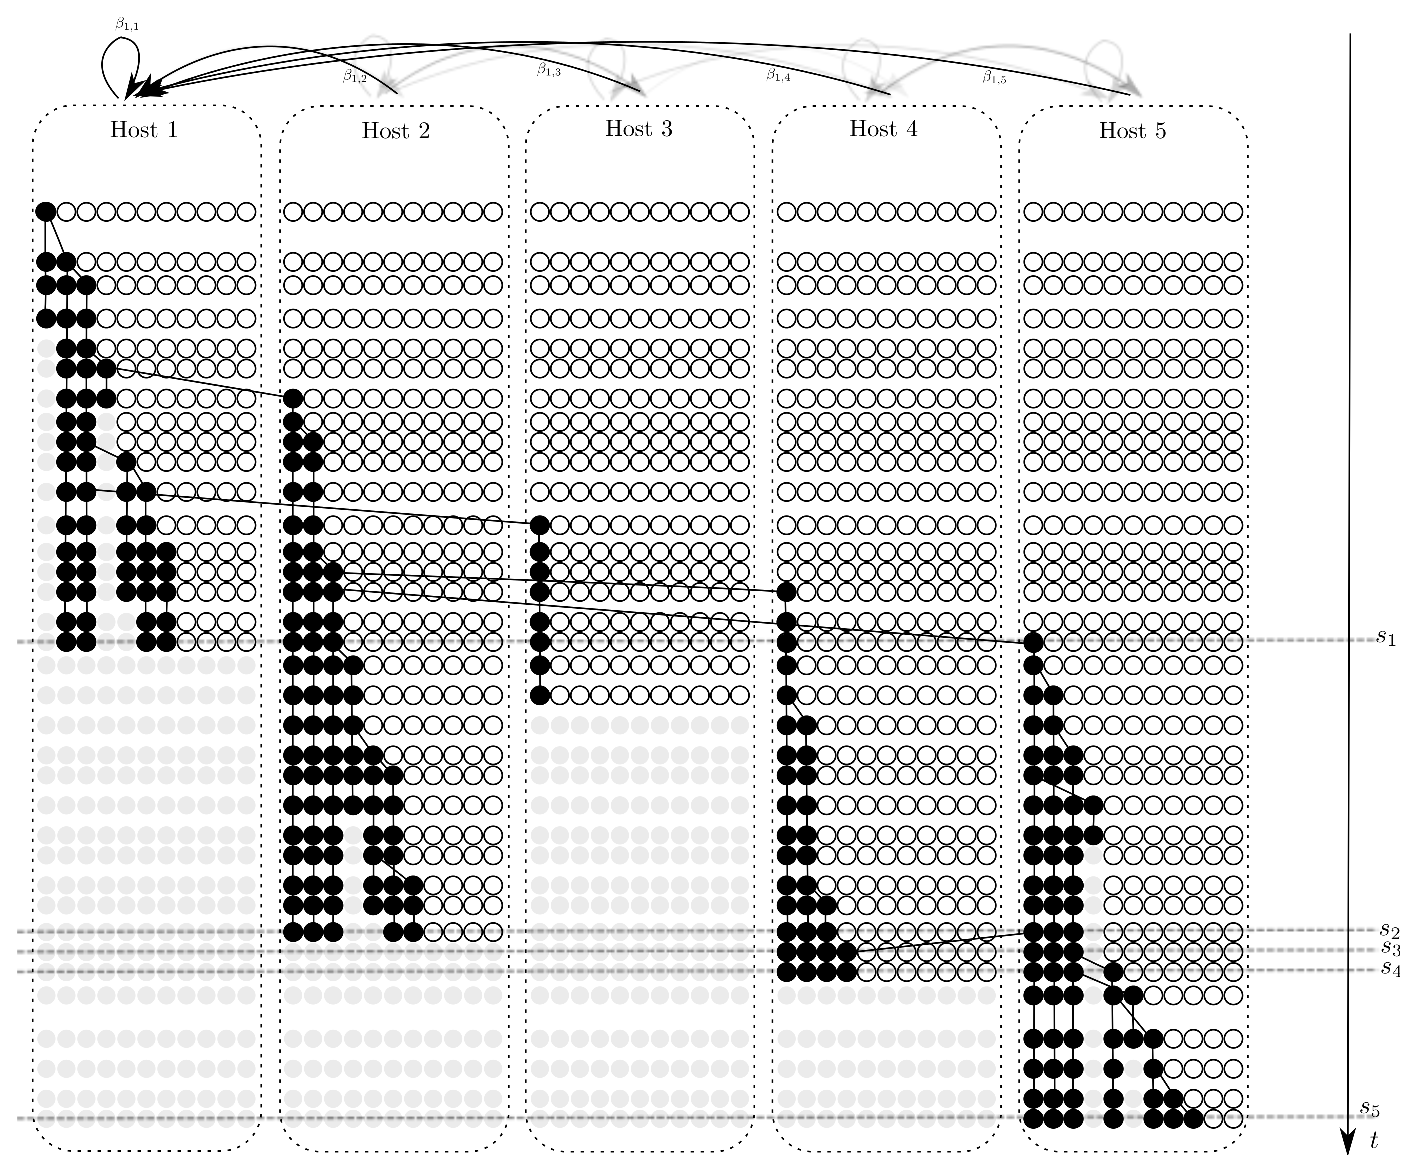
\includegraphics[width=0.8\textwidth]{model_1.eps}
\caption{Generation of genealogy for intrahost populations for $5$ hosts, observed at times $s_1$,...,$s_5$. Each host contains $N=11$ particles, which can be susceptible (white), infected (black), or recovered (grey). Initially (first row) all the particles are susceptible, except for $1$ infected in host $1$. The particles evolve according to the stochastic SIR process detailed in (\ref{eq:sirprocess}). Each infection is a birth event where the parent is chosen at random, and a recovery event is a death event for a randomly chosen infected particle.
}\end{figure}
Given the set of genetic sequences $\mathcal{D} = \{\mathbf{D}_1,...,\mathbf{D}_{N_h}\}$, observed at times $\mathbf{S} = \{s_1,...,s_{N_h}\}$ respectively, denote the underlying genealogy as $\mathcal{G}$. 
For a given $\mathcal{G}$, and mutation model, we can calculate the probability of $\mathcal{D}$ as shown in the next section. 
\subsection{Mutation model}
Associated with each leaf node of $\mathcal{G}$ is a nucleotide sequence (denote a sequence as $d_{h,i}$ ($h$ = host, $i$=sequence number in $h$'s viral population) . A likelihood can be calculated for the sequences at the tips of the tree ; we use the standard finite-sites selection-neutral likelihood framework with a general time-reversible (GTR) substitution model. Suppose that each of the sequences has length $L$, and at each site $l$ each base character in the sequence can take on values in the set $\mathcal{C}=\{A,C,G,T\}$. We use a mutation model that assumes that each site mutates in forward time according to a Poisson jump process, parameterised by a ($4 \times 4$) rate matrix $\mathbf{Q}$ where $\mathbf{Q}_{ij}$ is the instantaneous rate for the transition from character $i$ to character $j$ (A=$1$, C=$2$, G=$3$, T=$4$). The time units of the rates in $\mathbf{Q}$ are chosen such that the mean number of mutations per unit time occurring at a site is equal to $1$, and we scale this with parameter $\mu$, which represents the mean number of mutations per calendar unit at a site. 
To derive the likelihood, we consider an edge between parent $i$ and child $j$, $e_{ij}$ in $\mathcal{G}$. $j$ is a direct descendant of $i$, but the sequences $D_i$ and $D_j$ may be different if a mutation has occurred along the branch between $i$ and $j$. In this framework, the probability of a character at site $l$ in child $j$, given parent $i$, is expressed as $P(D_{j,l} = c' | D_{i,l} = c)=[\exp(-\mathbf{Q}\mu|e_{ij}|)]_{c,c'}$, for $c,c' \in \mathcal{C}$, and $|e_{ij}|$ is the edge length between $i$ and $j$. 

Let $\mathcal{D}$ denote the set of sequences associated with the tree tips, and $\mathcal{D}_A$ denote the (unknown) sequences associated with the ancestral / interior nodes. The probability for any particular set of sequences $\{\mathcal{D}, \mathcal{D}_A\}$ to be realised at the nodes of tree $\mathcal{G}$ is given by:
\begin{eqnarray}
P(\{\mathcal{D}, \mathcal{D}_A\}\mid \mathcal{G},\mu)=\prod_{\{i,j\}\in e} \prod_{l=1}^L [\exp(-\mathbf{Q}\mu|e_{ij}|)]_{D_{i,l},D_{j,l}}\label{eq:mut1}
\end{eqnarray}
We can integrate over the unknown $\mathcal{D}_A$ by summing over all sets of possible ancestral sequences $\mathbf{D}_A$.
\begin{eqnarray}
P(\mathcal{D}\mid \mathcal{G},\mu)=\sum_{\mathcal{D}_A \in \mathbf{D}_A} P(\{\mathcal{D}, \mathcal{D}_A\}\mid \mathcal{G},\mu)\label{eq:mut2}
\end{eqnarray}
which can be evaluated using a pruning algorithm \cite{felsenstein:1981}. 
\subsection{Generating the genealogy}
A genealogy $\mathcal{G}$ which gives rise to $\mathcal{D}$ will have $\sum_i P_i$ tips (the number of sequences), where each host's set of tips end at the corresponding sampling times $s_1,...,s_{N_h}$. Since a bifurcating tree is assumed, there are $(\sum_i P_i)-1$ interior nodes, which bifurcate at unknown times $\mathbf{b}=\{b_1,...,b_{(\sum_i P_i)-1}\}$. The genealogy can be completely specified by the bifurcation times, and the topology $\mathcal{T}$ ; $\mathcal{G}=\{\mathbf{b}, \mathcal{T}\}$. The following describes the generation of $\mathbf{b}$, through simulating SIR dynamics.
\subsubsection{Intrahost population trajectories}
For host $h$, we model the intrahost viral population as following SIR (susceptible, infected, recovered) dynamics. Let $S_h(t), I_h(t)$ and $R_h(t)$ denote random variables for the 
number of susceptible, infected, and immune `particles' respectively, where $S_h(t) + I_h(t) + R_h(t) = N$, where $N$ is the size of the viral population. We assume the following transition probabilities:
\begin{eqnarray}
P(\Delta S_h(t) &=& i, \Delta I_h(t) = j \mid S_1(t), I_1(t),..., S_{N_h}(t), I_{N_h}(t)) \label{eq:sirprocess}\\
&=& \left\{\begin{tabular}{l l l}
$\frac{\beta_{h,h'}}{N}S_h(t)I_{h'}(t)\Delta t + o(\Delta t)$, \hspace{0.4cm} & $h= h' : (i,j)=(-1,1)$ &  \\ 
& $h \neq h' : (i,j)=(-k_{h'}(t),k_{h'}(t))$ & \\
$\gamma I_h(t) \Delta t + o(\Delta t)$, & $(i,j)=(0,-1)$ & \nonumber\\
$1 - (\sum_k \frac{\beta_{h,k}}{N}S_h(t)I_k(t)\Delta t $ &  &\\
$+ \gamma I_h(t) \Delta t) + o(\Delta t)$, & $(i,j)=(0,0)$ &
\end{tabular}\right.
\end{eqnarray}
where $k_h$ is the number of particles that is transmitted from host $h$. We generate $k_h$ from a Binomial distribution $\textrm{Bin}(N, \phi_K)$

We generate the intrahost population trajectories via the Gillespie algorithm. There are $N_h(N_h+1)$ possible events:
$N_h \times N_h$ birth / infection events, and  $N_h$ death / recovery events. Denote their rates by $N_h \times (N_h+1)$ matrix $\mathbf{E}(t)$,
where $\mathbf{E}_{i,j}(t)=\frac{\beta_{i,j}}{N}S_i(t)I_j(t)$ is the rate at which host $j$ infects host $i$, and $\mathbf{E}_{i,N_h+1} = \gamma I_i(t)$ is the death rate in host $i$.

We keep track of the events in a matrix $\mathbf{T}$, where the $i$th row (corresponding to the $i$th event) is $\mathbf{T}_i=\{t_i, h_a, h_b, v\}$, where $t_i$ is the time of the event,
$v$ is the type of event $v \in \{-1,1\}$ (death, birth respectively) from host $h_b$ to $h_a$. See Algorithm \ref{alg:pts}.
\begin{algorithm}
\caption{Population trajectory sampling \label{alg:pts}}
\begin{algorithmic}
\STATE $t\gets 0$
\STATE $\mathbf{I}(0)\gets\{I_1(0)=1, I_2(0)=0, ..., I_{N_h}=0\}$
\STATE $\mathbf{S}(0)\gets\{S_1(0)=N-1, I_2(0)=N, ..., I_{N_h}=N\}$
\WHILE{$\sum_k I_k(t) > 0$}
\STATE Generate $k_h$
\STATE $t_e \sim \textrm{Exp}(\sum_k \frac{\beta_{h,k}}{N}S_h(t)I_k(t) + \gamma I_h(t))$ \COMMENT{Draw time until next event}
\STATE $e \sim \text{Categorical}(\mathbf{E}(t+t_e))$  \COMMENT{Draw event}
\STATE $t \gets t+t_e$
\STATE Update $\mathbf{I}(t), \mathbf{S}(t), \mathbf{T}$, based on $e$.
\ENDWHILE
\end{algorithmic}
\end{algorithm}

\subsubsection{Intrahost population trajectories given the data}

Given the sampling times $\{s_1,...,s_{N_h}\}$, and assuming that $P_h$ infected lineages in host $h$  are removed after sampling at time $s_h$, we modify the algorithm as shown in Algorithm \ref{alg:ptsd}.
\begin{algorithm}
\caption{Population trajectory sampling given data \label{alg:ptsd}}
\begin{algorithmic}
\STATE $t\gets 0$
\STATE $\mathbf{I}(0)\gets\{I_1(0)=1, I_2(0)=0, ..., I_{N_h}=0\}$
\STATE $\mathbf{S}(0)\gets\{S_1(0)=N-1, I_2(0)=N, ..., I_{N_h}=N\}$
\WHILE{$\sum_k I_k(t) > 0$}
\STATE Generate $k_h$
\STATE $t_e \sim \textrm{Exp}(\sum_k \frac{\beta_{h,k}}{N}S_h(t)I_k(t) + \gamma I_h(t))$ \COMMENT{Draw time until next event}
\FOR{$h=1$ to $N_h$}
{\IF{$t+t_e>s_h$} 
\STATE $I_h(t+t_e)\gets I_h(t+t_e) - P_h$ 
\STATE Update $\mathbf{T}$
\ENDIF}
\ENDFOR
\STATE $e \sim \textrm{Categorical}(\mathbf{E}(t+t_e))$  \COMMENT{Draw event after updating $\mathbf{E}$}
\STATE $t \gets t+t_e$
\STATE Update $\mathbf{I}(t), \mathbf{S}(t), \mathbf{T}$, based on $e$.
\ENDWHILE
\end{algorithmic}
\end{algorithm}
In order to simulate $\mathcal{G}$ which gives a non-zero likelihood $p(\mathcal{D}\mid \mathcal{G}, \mu)$, we require the number of infected particles in the hosts when they are observed at times $\mathbf{S}=\{s_1,...,s_{N_h}\}$ to be consistent with the data $\mathcal{D}$.  We write the prior for the set of infected population trajectories $\mathbf{I}(t)$ as:
\begin{eqnarray}
p(\mathbf{I}(t) \mid  \gamma, \{\beta_{1,1},...,\beta_{N_h,N_h}\}, N, \phi_K, t_{off})
\end{eqnarray}
which can be sampled via simulation by Algorithm \ref{alg:ptsd}, where $t_{off}$ denotes the time between the start of the trajectory and the first sampling time. Denoting $P_i$ as the number of sequences in host $i$, sampled at time $s_i$, we only accept the simulated trajectory if the number of surviving lineages (tips) at times $s_1,...,s_{N_h}$ in hosts $1,...,N_h$ are $\{ \geq P_1,..,\geq P_{N_h}\} $ respectively.
%The likelihood of $\mathcal{G} = \{\{b_1,...,b_{(\sum_i P_i)-1}\},\mathcal{T}\}$ under the data (the number of sequences and their time of sampling) is given by:
%\begin{eqnarray}
%p(P_1,...,P_{N_H} \mid \mathcal{G}, \mathbf{S}) \label{eq:113}
%\end{eqnarray}
%which will be $1$ if the number of surviving lineages (tips) at times $s_1,...,s_{N_h}$ in hosts $1,...,N_h$ are $\{ \geq P_1,..,\geq P_{N_h}\} $ respectively, and $0$ otherwise.
%To draw a sample from 
%\begin{eqnarray}
%p(\{\mathcal{G} \mid \gamma, \{\beta_{1,1},...,\beta_{N_h,N_h}\}, N, N_h, P_1,...,P_{N_H}, \mathbf{S}) \label{eq:ll2}
%\end{eqnarray}
%we draw $\mathcal{G}$ according to $I(t)$, from the SIR process, and accept the sample if (\ref{eq:ii3}=$1$).


\subsubsection{Reconstructed tree and bifurcation times}
We relate the infected population trajectory $\mathbf{I}(t)$ to a genealogical tree: each birth / infection event is a bifurcation event (a lineage splits in two), and recovery is the death of a lineage. Each lineage corresponds to an infected particle, and for each event, a particle is picked at random.
See Figure \ref{fig:tree1}. We then remove extinct lineages to get a 'reconstructed tree' (see Figure \ref{fig:tree2}). This results in a genealogy that underlies the set of observed sequences  $\mathbf{G}$, generated by a birth-death process, where the birth and death rates are governed by SIR dynamics (\ref{eq:sirprocess}), with  $\sum_i^{N_h} P_i - 1$ bifurcations / coalescent events at times $\mathbf{b}=\{b_1,...,b_{(\sum_i P_i)-1}\}$, and the topology $\mathcal{T}$ is partially defined on a host-host level, since we know which host each particle is in. Let's record the bifurcation times $\mathbf{b}$ and partial topology in matrix $\mathbf{T}^R$, where the $i$th row corresponds to the $i$th bifurcation event: $\mathbf{T}^R_i=\{b_i, H_p, H_{c_1}, H_{c,2}\}$, where $H_p, H_{c_1}, H_{c,2}$ are the hosts of the parent, and two children. We can generate the full topology from $\mathbf{T}_R$. The prior for $\mathcal{G}$ for $N_h$ hosts under the SIR intrahost dynamics is given by 
\begin{eqnarray}
p(\mathcal{G}\mid \mathbf{I}(t)) \label{eq:ll1}
\end{eqnarray}
and we can evaluate this by using a coalescent tree approximation in the following section.
\section{Tree likelihood}
Here, we derive a likelihood for a genealogy given a sample from an SIR trajectory. Given the population of infected in the $N_H$ hosts $\mathbf{I}(t) = \{I_1(t), I_2(t),...,I_{N_H}(t)\}$,  and the number of sampled lineages in the hosts as $\mathbf{n}(t)=\{n_1(t), n_2(t), ... , n_{N_H}(t)\}$, we want to write the likelihood for the ancestral tree $\mathcal{G}$ of the observed sequences.  $\mathbf{I}(t)$ is a stepwise function which evolves according to the following transition probabilities from equation \ref{eq:sir process}:
Firstly, we note that the distribution of the waiting time $g_n$ between $t_{n+1}$ and $t_n$, (where $t_n$ is the time of coalescence into $n$ lineages) with rate of coalescence $\lambda$, is given by:
\begin{eqnarray}
p(g_n\mid t_n) = \textrm{Exp}(\lambda) = \lambda e^{-\lambda} 
\end{eqnarray}
The rate of coalescence is dependent on the population size ;  for instance, Volz \cite{Volz2009} writes the rate of coalescence for a SIR model within one host as:
\begin{eqnarray}
\lambda_t = \frac{{n \choose 2}}{{I(t) \choose 2}}  \frac{\beta S(t)}{N}I(t)
\end{eqnarray}
This has the interpretation that the rate of coalescence at time $t$ is the overall transmission rate in the population of size $N$ multiplied by the probability of observing a transmission in the $n$ ancestors. We can extend this idea to our model with multiple hosts, and transmission events.

We can specify the ancestral tree $\mathcal{G}$ by the following events $\mathcal{E}=\{\}$: 
\subsubsection{A coalescent event between two observed lineages within a host}
The rate of coalescence where $i=j$, and both lineages are observed is given by:
\begin{eqnarray}
\lambda_{ii}^o(t) =  \frac{{n_i(t) \choose 2}}{{I_i(t) \choose 2}}  \frac{\beta_{ii} S_i(t')}{N}I_i(t')
\end{eqnarray}
where $t'$ is the time immediately before $t$
\subsubsection{Transmission of an observed lineage between two hosts}
In the model, $k$ lineages are transmitted from host $i$ to $j$ at rate $\frac{\beta_{ji}S_j(t)}{N}I_i(t)$, if $S_j(t) \geq k, I_i(t) \geq k$. We can scale the transmission rate so that the rate when at least one of the observed lineages moves from host $i$ to host $j$ is given by : 
%\begin{eqnarray}
%\lambda_{ij}^o(t) =  \frac{(I_j(t) - n_j(t))!(I_j(t) - k)!)}{(I_j(t) - n_j(t) - k)! I_j!}  \frac{\beta_{ji} S_j(t')}{N}I_i(t')
%\end{eqnarray}
%\begin{eqnarray}
%\lambda_{ij}^o(t) =  \sum_k p(k) \frac{{I_j(t) \choose k} - {I_j(t)  - n_j(t) \choose k}  )}{{I_j(t) \choose k}}  \frac{\beta_{ji} S_j(t')}{N}I_i(t')
%\end{eqnarray}
\begin{eqnarray}
\lambda_{ij}^o(t) =  \frac{{I_j(t) \choose k} - {I_j(t)  - n_j(t) \choose k}  )}{{I_j(t) \choose k}}  \frac{\beta_{ji} S_j(t')}{N}I_i(t')
\end{eqnarray}
where $k$ is drawn from a binomial distribution.
%Let's denote a coalescent event as $e_n = \{t_n, o_i, o_j\} $ where $t_n$ is the branching time of $n$ ancestors to $n+1$,, and $o_i$ and $o_j$ are binary variables which indicate whether each lineage is observed. 
\subsection{Calculation of likelihood}
We can calculate the likelihood of $\mathcal{G}$ by dividing it into intervals $g_i$ between the events in $\mathcal{E} $ (i.e. $g_i$ is the waiting time between the $i-1$th and $i$th event in $\mathcal{E}$), and then taking the product of the likelihood over all intervals. Denote the event times by $t_i$. $\mathbf{I}(t)$ is a stepwise function ; denote the change points in interval $g_i$ by  $\mathbf{s} = \{s_1, ... , s_{T_i}\}$ (moving backwards in time, $s_1=t_i$, $s_{T_i}=t_{i-1}$).
\subsubsection{Event times}
At $t_n$, going back in time, the waiting time $g_n$ until the {\it next} event in $\mathcal{E}$ is given by:
\begin{eqnarray}
p(g_n \mid t_n) &=& \lambda^o(t_n - g_n) e^{-\int_{t=t_n}^{t_n - g_g} \lambda^o(t)dt} \nonumber\\
&=& \lambda^o(s_{T_i-1}) e^{-\sum_{i=1}^{T_i-1} \lambda^o(s_i)(s_{i+1} - s_i)}
\end{eqnarray}
where 
\begin{eqnarray}
\lambda^o(t) = \sum_{i,j}\lambda_{ij}^o(t)
\end{eqnarray}
\subsubsection{Tree topology}
The probability of a tree topology $\tau_n$ in interval $g_n$ is the product of the probability of the event that occurs, and the probability of the tree topology of that event.
The probability of one of the events in $\mathcal{E}$ occurring is given by:
\begin{eqnarray}
p(\mathcal{E}_{ij} \mid g_n) = \frac{\lambda_{ij}^o(t_n - g_n)}{\lambda^o(t_n - g_n)}  \nonumber \\
\end{eqnarray}
and the topology probability for  $i=j$
\begin{eqnarray}
p(\tau_n \mid \mathcal{E}_{ii}, g_n) = \frac{1}{{n_i (t_n)\choose 2}} 
\end{eqnarray}
For $i \neq j$, given that $m$ {\it observed} lineages from host $j$ coalesce with $m$ lineages from host $i$, of which $m'$ are observed:
\begin{eqnarray}
p(\tau_n \mid \mathcal{E}_{ji}, g_n) = \frac{ {I_i(t_n) - n_i(t_n) \choose m - m'}(m-m')!}{{n_j (t_n)\choose m} \frac{I_i(t_n)!}{(I_i(t_n) - m)!}} 
\end{eqnarray}
The denominator is the number of topologies if there are $m$ coalescent events between hosts $i$ and $j$, and the numerator is the number of ways of picking a particular set of $m'$ observed lineages from host $i$, and $m-m'$ unobserved. 
%\begin{eqnarray}
%p(\mathcal{E}_{ij}) = \frac{\lambda_{ij}^o}{\lambda^o(t_n - g_n)}  \nonumber \\
%p(g_n, i, j \mid t_n)&=& \frac{\lambda_{ij}^o}{\lambda^o(t_n - g_n)} p(g_n \mid t_n)\nonumber\\
%&=& \lambda_{ij}^o(t_n - g_n) e^{-\int_{t=t_n}^{t_n - g_n} \lambda^o(t)dt}
%\end{eqnarray}
Putting everything together, the likelihood is calculated by:
\begin{eqnarray}
\mathcal{L} = \prod_n p(\tau_n, \mathcal{E}_n, g_n \mid t_n)
\end{eqnarray}

[Figure here]
\section{Inference}
We want to infer the parameters of the SIR model $\Theta_{I} = \{\gamma$, $\boldsymbol{\beta}= \{\beta_{1,1},...,\beta_{N_h,N_h}\}, t_{off}, \theta_K\}$, the mutation model $\Theta_{\mu} = \{\mu\}$, and the underlying genealogy $\mathcal{G}$ through targeting the joint posterior density:
\begin{eqnarray}
p(\Theta_{I}, \Theta_{\mu}, \mathcal{G}, \mathbf{I} \mid \mathcal{D})\propto p(\mathcal{D}\mid \mathcal{G}, \Theta_{\mu})p(\mathcal{G}\mid \mathbf{I}) p(\mathbf{I} \mid \Theta_{I}) p(\Theta_{\mu}) p(\Theta_{I})
\end{eqnarray}
We describe a Monte Carlo scheme for sampling from the posterior density through constructing a Markov chain, where successive samples from the state $\Theta=\{\Theta_{I}, \Theta_{\mu}, \mathcal{G}, \mathbf{I} \}$ converges to a sample of the posterior. We use a Metropolis-Hastings algorithm to generate moves around the parameter space, where we define a set of $M$ random operations on $\Theta$, $q_m(\Theta'\mid \Theta)$, $m=1,..,M$. An operation/move $m'$ is chosen at random, then a new value $\Theta'$ is drawn from  $q_{m'}(\Theta'\mid \Theta)$, and accepted with probability (unless defined otherwise) 
\begin{eqnarray}
\alpha_{m'}(\Theta',\Theta)=\textrm{min}\left(1,\frac{p(\mathcal{D}\mid \Theta')p(\Theta')}{p(\mathcal{D}\mid \Theta)p(\Theta)} \frac{q(\Theta\mid\Theta')}{q(\Theta'\mid\Theta)}\right)
\end{eqnarray}
\subsection{Mutation model parameters $\Theta_{\mu}$} 
\subsubsection{Move $1$: $\mu$}
In updating $\mu$, based on the current state $\Theta$, we are drawing from $p(\mu\mid\mathcal{D},\mathcal{G}) \propto p(\mathcal{D}\mid \mathcal{G}, \mu)p(\mu)$. We use a Gaussian proposal density:
\begin{eqnarray}
\{\gamma', \boldsymbol{\beta}', \mu', \mathcal{G}'\}\leftarrow\{\gamma, \boldsymbol{\beta}, \mu+\delta, \mathcal{G}\}
\end{eqnarray}
where $\delta\sim\mathcal{N}(0,\sigma_{\mu}^2)$, such that 
\begin{eqnarray}
q_1(\Theta'\mid\Theta) = \mathcal{N}(\mu'-\mu,0,\sigma_{\mu}^2)
\end{eqnarray}
Since this is a symmetrical proposal density, the move is accepted with acceptance probability:
\begin{eqnarray}
\alpha_{1}(\Theta',\Theta)=\textrm{min}\left(1,\frac{p(\mathcal{D}\mid \mathcal{G}, \mu')p(\mu')}{p(\mathcal{D}\mid \mathcal{G}, \mu )p(\mu)} \right)
\end{eqnarray}
\subsection{Genealogy $\mathcal{G}$} 
%When generating the genealogy $\mathcal{G}$ from the SIR model parameters, the information about the reconstructed tree is stored in matrix  $\mathbf{T}^{R}$, where the $i$th row (corresponding to the $i$th event) is  $\mathbf{T}^R_{i} = \{b_i, H_p, H_{c_1}, H_{c_2}\}$, where columns $2$, $3$, and $4$ are the hosts of the parent, child $1$ and child $2$ respectively. So we are simulating $p(\mathbf{T}^R\mid \gamma, \boldsymbol{\beta}, N, N_h, \mathbf{P}, \mathbf{S})$. Using the host-host information in $\mathbf{T}^R$, we can create the full topology to get the final genealogy $p(\mathcal{G}\mid \mathbf{T}^R)$, by assuming that all configurations corresponding with $\mathbf{T}^R$ are equally likely.   

When generating the genealogy $\mathcal{G}$ from the SIR parameters, the trajectory of the infected population sizes $\mathbf{I}$ is simulated, and then the genealogy is constructed by simulating an ancestral tree for all the sequences from $p(\mathcal{G} \mid \mathbf{I})$  such that a sample is generated from $p(\mathcal{G}, \mathbf{I} \mid \Theta_{I})$.
We define three possible proposal mechanisms. Move $2$ proposes a new genealogy based on the current SIR parameters and topology. Moves $3$ and $4$ propose changes to the topology $\mathcal{T}$.

\subsubsection{Move $2$: $\mathcal{G}, \mathbf{I}$}
We then simulate the genealogy $\mathcal{G}'$ and trajectory $\mathbf{I}$, from  $p(\mathcal{G}, \mathbf{I} \mid \Theta_{I})$.  Basing the new proposed genealogy on the current topology tries to ensures that the new proposal is close in tree space. The move is accepted with probability 
\begin{eqnarray}
\alpha_{2}(\Theta',\Theta)=\textrm{min}\left(1,\frac{p(\mathcal{D}\mid \mathcal{G}', \mu) p(\mathcal{G}', \mathbf{I}' \mid \Theta_{I})}{p(\mathcal{D}\mid \mathcal{G}, \mu ) p(\mathcal{G}, \mathbf{I} \mid \Theta_{I})} \right)
\end{eqnarray}
\subsubsection{Move 3: $\mathcal{T}$}
This proposal changes the topology of the genealogy $\mathcal{G}$, using "narrow exchange", similar to the move detailed in \cite{Drummond:2002it}. This move picks two subtrees at random under the constrain that they have an aunt-niece relationship. These two subtrees are swapped as long as doing so does not require any modifications to the node heights and the host-host relationships between nodes. 
\subsubsection{Move 4: $\mathcal{T}$}
This proposal changes the topology of the genealogy $\mathcal{G}$, using "wide exchange". This move picks two subtrees at random. These two subtrees are swapped as long as doing so does not require any modifications to the node heights and the host-host relationships between nodes. 
\subsection{SIR parameters $\Theta_{I}$}
We propose a new value for the $\Theta_{I}'$, then simulate a new $\mathcal{G}', \mathbf{I}'$,  which is accepted with probability 
\begin{eqnarray}
\alpha_{5}(\Theta',\Theta)=\textrm{min}\left(1,\frac{p(\mathcal{D}\mid \mathcal{G}', \mu) p(\mathcal{G}', \mathbf{I}' \mid \Theta_{I}')p(\Theta_{I}')}{p(\mathcal{D}\mid \mathcal{G}, \mu ) p(\mathcal{G}, \mathbf{I} \mid \Theta_{I})p(\Theta_I)} \right)
\end{eqnarray}


\subsection{Old moves (phased out)}
\subsubsection{Move $3$: $\boldsymbol\beta$}
$\boldsymbol\beta$ is an $N_h \times N_h$ matrix which defines the transmission rates within and between the $N_h$ hosts. Sampling $\boldsymbol\beta$ requires a draw from $p(\boldsymbol{\beta}\mid\mathcal{G},\gamma,N,N_h)\propto p(\mathcal{G}\mid\gamma, \boldsymbol{\beta},N,N_h)p(\boldsymbol{\beta})$. However, since we can't evaluate the likelihood $p(\mathcal{G}\mid\gamma, \boldsymbol{\beta},N,N_h)$, so have to resort to an approximation, through simulation. We use a method of approximate Bayesian computation (ABC) ; the likelihood function is approximated through simulation - and the simulated genealogy $\mathcal{G}^*$ is accepted if it is close to the current genealogy $\mathcal{G}$. We use a Gaussian proposal density for each element of $\boldsymbol{\beta}$, (after transforming to log space to keep the parameter values positive) such that:
\begin{eqnarray}
q_3(\Theta',\Theta)=\prod_{i,j} \mathcal{N}(\log \beta_{i,j}' - \log \beta_{i,j}, 0 , \sigma_{\beta_{i,j}}^2)
\end{eqnarray}
\begin{algorithm}
\caption{ABC for $\boldsymbol\beta$ \label{alg:beta}}
\begin{algorithmic}
\STATE Propose a move $\boldsymbol{\beta}'\gets \boldsymbol{\beta}$ using $q_3$
\STATE Generate $\mathcal{G}^*$ using $p(\mathcal{G}^*\mid \gamma, \boldsymbol{\beta}', N, N_h, \mathbf{P}, \mathbf{S})$
\STATE Calculate distance $\rho(\mathcal{G},\mathcal{G}^*)$
\IF{$\rho(\mathcal{G},\mathcal{G}^*) \leq \epsilon$}
\STATE Calculate $\alpha_{3}(\Theta',\Theta)=\textrm{min}\left(1,\frac{p(\boldsymbol{\beta}')}{p(\boldsymbol{\beta}'} \right)$
\STATE Accept $\boldsymbol{\beta}'$ with probability $\alpha_3$.
\ENDIF
\end{algorithmic}
\end{algorithm}
For the distance measure $\rho$, the average Euclidean distance between the $(\sum P_i) -1$ bifurcation times are used: $\rho = \frac{1}{(\sum P_i) -1}||\mathbf{b}'-\mathbf{b}||$.
\subsubsection{Move $4$: $\gamma$}
We use a similar scheme to Move $3$ to generate a new value for $\gamma$, the death rate of the SIR process.
\begin{eqnarray}
q_4(\Theta',\Theta)= \mathcal{N}(\log \gamma' - \log \gamma, 0 , \sigma_{\gamma}^2)
\end{eqnarray}
\begin{algorithm}
\caption{ABC for $\gamma$ \label{alg:gamma}}
\begin{algorithmic}
\STATE Propose a move $\gamma'\gets \gamma$ using $q_4$
\STATE Generate $\mathcal{G}^*$ using $p(\mathcal{G}^*\mid \gamma', \boldsymbol{\beta}, N, N_h, \mathbf{P}, \mathbf{S})$
\STATE Calculate distance $\rho(\mathcal{G},\mathcal{G}^*)$
\IF{$\rho(\mathcal{G},\mathcal{G}^*) \leq \epsilon$}
\STATE Calculate $\alpha_{4}(\Theta',\Theta)=\textrm{min}\left(1,\frac{p(\gamma')}{p(\gamma)} \right)$
\STATE Accept $\gamma'$ with probability $\alpha_4$.
\ENDIF
\end{algorithmic}
\end{algorithm}
using the same distance measure as before.





\begin{figure}[h]
\centering
\subfigure[Intrahost genealogies for two hosts]{
\includegraphics{tree1.eps}
\label{fig:tree1}
}\\
\subfigure[Reconstructed intrahost genealogies for (a)]{
\includegraphics{tree2.eps}
\label{fig:tree2}
}
\caption{Possible underlying genealogy for two infected hosts with viral populations of size 5 and 3.}
\end{figure}

\section{Inference using particle MCMC}
When making proposing a new genealogy $\mathcal{G}^*$, the acceptance rate will be low, because the branch lengths and inter-host topology are 
constructed from independent samples of the underlying SIR process: simulated from $p(\mathbf{I}^* \mid \Theta_I^*)$ and then $p(\mathcal{G}^* \mid \mathbf{I}^*)$. 
The samples of the genealogy are not guaranteed to be close in tree space. A better inference scheme would be to ensure that the proposed genealogies are consistent with the data,
by simulating from $p(\mathbf{I}^* \mid \Theta_I^*)$, and then from $p(\mathcal{G}^* \mid \mathbf{I}^*, \mathcal{D})$. 

To sample from $p(\mathcal{G}^* \mid \mathbf{I}^*, \mathcal{D})$, we use a particle filter, described below. The proposed $\{\mathcal{G}^*, \mathbf{I}^* , \Theta_I^*\}$ is accepted 
with the Metropolis Hastings ratio:
\begin{eqnarray}
\alpha = \frac{\hat{p}(\mathcal{D} \mid \Theta_I^*)p(\Theta_I^*)q(\Theta_I\mid \Theta_I^*)}{\hat{p}(\mathcal{D} \mid \Theta_I)p(\Theta_I)q(\Theta_I^*\mid \Theta_I) }
\end{eqnarray}
where $\hat{p}(\mathcal{D} \mid \Theta_I)$ is the particle filter's estimate of marginal likelihood. 

\subsection{Particle filter for trees}
We use the notation: $g_n^k$ to denote a genealogy of the first $n$ sequences from $\mathcal{D}$, with index $k$, and the associated trajectory by $I_n^k$. The particle cloud is
given by $\{\mathbf{g}_n, \mathbf{I}_n\}=\{g_n^k,  I_n^k \mid k=1,..,N_p\}$  

\section{Summary}
\begin{tabular}{|l|l|}
\hline 
\multicolumn{2}{|c|}{Data}\\
\hline
Number of hosts & $N_h$  \\
Number of sequences in hosts & $P_1,...,P_{N_h}$ \\
Sequences & $\mathcal{D}=\{\mathbf{d}_{1,1},...,\mathbf{d}_{1,P_1}\},...,\{\mathbf{d}_{N_h,1},...,\mathbf{g}_{1,P_{N_h}}\} $ \\
Time of sequences/ host sampling& $\mathbf{S}=\{s_1,...,s_{N_h}\}$ \\
Number of yards & $N_y$  \\
Fraction of yard infected & $\alpha_1,...,\alpha_{N_y}$ \\
\hline 
\multicolumn{2}{|c|}{SIR model parameters}\\
\hline
Infection rates for particles from  & $\beta_{i,j}, i \in 1,...,N_h, j \in 1,...,N_h$ \\
host $i$ and host $j$ & \\
Recovery rate for particles in host $i$ & $\gamma$ \\
Initial number of susceptible particles in each host & $N$ \\
\hline 
\multicolumn{2}{|c|}{SIR model output}\\
\hline
SIR population trajectories & $S(t), I(t), R(t)$ \\
Summary of infection/ recovery events and times & $\mathbf{T}$, $\mathbf{T}_i=\{\textrm{time of event, from, to, event type} \}$ \\
Summary of infection events & $\mathbf{T}^R$, $\mathbf{T}^R_i=\{b_i, H_p,H_{c_1}, H_{c_2}] \}$ \\
from reconstructed tree & \\
\hline 
\multicolumn{2}{|c|}{Genealogy $\mathcal{G}$}\\
\hline
Number of tips & should be $\sum_i^{N_h}P_i$ \\
Bifurcation/'significant' infection times & $b_1,...,b_{\sum_i^{N_h}P_i}$ \\
derived from SIR model&  \\
Topology & $\mathcal{T} $\\
\hline
\multicolumn{2}{|c|}{Mutation model}\\
\hline
Mutation rate & $\mu$ \\
Other parameters & relative rate matrix, genealogy $\mathcal{G}$ \\
\hline
\end{tabular}
\bibliography{phylodynamic}
\bibliographystyle{plain}
\end{document}
